\documentclass{ximera}


\graphicspath{
  {./}
  {1-1QuantitativeReasoning/}
  {1-2RelationsAndGraphs/}
  {1-3ChangingInTandem/}
  {2-1LinearEquations/}
  {2-2LinearModeling/}
  {2-3ExponentialModeling/}
  {3-1WhatIsAFunction/}
  {3-2FunctionProperties/}
  {3-3AverageRatesOfChange/}
  {4-1BuildingNewFunctions/}
  {4-2Polynomials/}
  {5-1RationalFunctions/}
   {5-2ExponentialFunctions/}
  {6-1Domain/}
  {6-2Range/}
  {6-3CompositionOfFunctions/}
  {7-1ZerosOfFunctions/}
  {7-XZerosOfPolynomials/}
  {7-2ZerosOfFamousFunctions/}
  {8-0Review/}
  {8-1FunctionTransformations/}
  {8-2SolvingInequalities/}
  {8-3FunctionTransformationsProject/}
  {9-1RightTriangleTrig/}
  {9-2TheUnitCircle/}
  {9-3TrigIdentities/}
  {10-1UnitCircleToFunctionGraph/}
  {10-2TrigFunctions/}
  {10-3SomeApplicationsOfTrig/}
  {11-1InverseFunctionsRevisited/}
  {11-2Logarithms/}
  {11-3InverseTrig/}
  {12-1SystemsOfEquations/}
  {12-2NonlinearSystems/}
  {12-3ApplicationsOfSystems/}
  {13-1SecantLinesRevisited/}
  {13-2Functions-TheBigPicture/}
  {14-1DisplacementVsDistance/}
  {1-1QuantitativeReasoning/exercises/}
  {1-2RelationsAndGraphs/exercises/}
  {../1-3ChangingInTandem/exercises/}
  {../2-1LinearEquations/exercises/}
  {../2-2LinearModeling/exercises/}
  {../2-3ExponentialModeling/exercises/}
  {../3-1WhatIsAFunction/exercises/}
  {../3-2FunctionProperties/exercises/}
  {../3-3AverageRatesOfChange/exercises/}
  {../5-2ExponentialFunctions/exercises/}
  {../4-1BuildingNewFunctions/exercises/}
  {../4-2Polynomials/exercises/}
  {../5-1RationalFunctions/exercises/}
  {../6-1Domain/exercises/}
  {../6-2Range/exercises/}
  {../6-3CompositionOfFunctions/exercises/}
  {../7-1ZerosOfFunctions/exercises/}
  {../7-XZerosOfPolynomials/exercises/}
  {../7-2ZerosOfFamousFunctions/exercises/}
  {../8-1FunctionTransformations/exercises/}
  {../12-1SystemsOfEquations/exercises/}
  {../8-3FunctionTransformationsProject/exercises/}
  {../8-0Review/exercises/}
  {../8-2SolvingInequalities/exercises/}
  {../8-3FunctionTransformationsProject/exercises/}
  {../9-1RightTriangleTrig/exercises/}
  {../9-2TheUnitCircle/exercises/}
  {../9-3TrigIdentities/exercises/}
  {../10-1UnitCircleToFunctionGraph/exercises/}
  {../10-2TrigFunctions/exercises/}
  {../10-3SomeApplicationsOfTrig/exercises/}
  {../11-1InverseFunctionsRevisited/exercises/}
  {../11-2Logarithms/exercises/}
  {../11-3InverseTrig/exercises/}
  {../12-1SystemsOfEquations/exercises/}
  {../12-2NonlinearSystems/exercises/}
  {../12-3ApplicationsOfSystems/exercises/}
  {../13-1SecantLinesRevisited/exercises/}
  {../13-2Functions-TheBigPicture/exercises/}
  {../14-1DisplacementVsDistance/exercises/}
}

\DeclareGraphicsExtensions{.pdf,.png,.jpg,.eps}

\newcommand{\mooculus}{\textsf{\textbf{MOOC}\textnormal{\textsf{ULUS}}}}

\usepackage[makeroom]{cancel} %% for strike outs

\ifxake
\else
\usepackage[most]{tcolorbox}
\fi


%\typeout{************************************************}
%\typeout{New Environments}
%\typeout{************************************************}

%% to fix for web can be removed when deployed offically with ximera2
\let\image\relax\let\endimage\relax
\NewEnviron{image}{% 
  \begin{center}\BODY\end{center}% center
}



\NewEnviron{folder}{
      \addcontentsline{toc}{section}{\textbf{\BODY}}
}

\ifxake
\let\summary\relax
\let\endsummary\relax
\newtheorem*{summary}{Summary}
\newtheorem*{callout}{Callout}
\newtheorem*{overview}{Overview}
\newtheorem*{objectives}{Objectives}
\newtheorem*{motivatingQuestions}{Motivating Questions}
\newtheorem*{MM}{Metacognitive Moment}
      
%% NEEDED FOR XIMERA 2
%\ximerizedEnvironment{summary}
%\ximerizedEnvironment{callout}
%\ximerizedEnvironment{overview} 
%\ximerizedEnvironment{objectives}
%\ximerizedEnvironment{motivatingQuestions}
%\ximerizedEnvironment{MM}
\else
%% CALLOUT
\NewEnviron{callout}{
  \begin{tcolorbox}[colback=blue!5, breakable,pad at break*=1mm]
      \BODY
  \end{tcolorbox}
}
%% MOTIVATING QUESTIONS
\NewEnviron{motivatingQuestions}{
  \begin{tcolorbox}[ breakable,pad at break*=1mm]
    \textbf{\Large Motivating Questions}\hfill
    %\begin{itemize}[label=\textbullet]
      \BODY
    %\end{itemize}
  \end{tcolorbox}
}
%% OBJECTIVES
\NewEnviron{objectives}{  
    \vspace{.5in}
      %\begin{tcolorbox}[colback=orange!5, breakable,pad at break*=1mm]
    \textbf{\Large Learning Objectives}
    \begin{itemize}[label=\textbullet]
      \BODY
    \end{itemize}
    %\end{tcolorbox}
}
%% DEFINITION
\let\definition\relax
\let\enddefinition\relax
\NewEnviron{definition}{
  \begin{tcolorbox}[ breakable,pad at break*=1mm]
    \noindent\textbf{Definition}~
      \BODY
  \end{tcolorbox}
}
%% OVERVIEW
\let\overview\relax
\let\overview\relax
\NewEnviron{overview}{
  \begin{tcolorbox}[ breakable,pad at break*=1mm]
    \textbf{\Large Overview}
    %\begin{itemize}[label=\textbullet] %% breaks Xake
      \BODY
    %\end{itemize}
  \end{tcolorbox}
}
%% SUMMARY
\let\summary\relax
\let\endsummary\relax
\NewEnviron{summary}{
  \begin{tcolorbox}[ breakable,pad at break*=1mm]
    \textbf{\Large Summary}
    %\begin{itemize}[label=\textbullet] %% breaks Xake
      \BODY
    %\end{itemize}
  \end{tcolorbox}
}
%% REMARK
\let\remark\relax
\let\endremark\relax
\NewEnviron{remark}{
  \begin{tcolorbox}[colback=green!5, breakable,pad at break*=1mm]
    \noindent\textbf{Remark}~
      \BODY
  \end{tcolorbox}
}
%% EXPLANATION
\let\explanation\relax
\let\endexplanation\relax
\NewEnviron{explanation}{
    \normalfont
    \noindent\textbf{Explanation}~
      \BODY
}
%% EXPLORATION
\let\exploration\relax
\let\endexploration\relax
\NewEnviron{exploration}{
  \begin{tcolorbox}[colback=yellow!10, breakable,pad at break*=1mm]
    \noindent\textbf{Exploration}~
      \BODY
  \end{tcolorbox}
}
%% METACOGNITIVE MOMENTS
\let\MM\relax
\let\endMM\relax
\NewEnviron{MM}{
  \begin{tcolorbox}[colback=pink!15, breakable,pad at break*=1mm]
    \noindent\textbf{Metacognitive Moment}~
      \BODY
  \end{tcolorbox}
}


\fi





%Notes on what envirnoment to use:  Example with Explanation in text; if they are supposed to answer- Problem; no answer - Exploration


%\typeout{************************************************}
%% Header and footers
%\typeout{************************************************}

\newcommand{\licenseAcknowledgement}{Licensed under Creative Commons 4.0}
\newcommand{\licenseAPC}{\renewcommand{\licenseAcknowledgement}{\textbf{Acknowledgements:} Active Prelude to Calculus (https://activecalculus.org/prelude) }}
\newcommand{\licenseSZ}{\renewcommand{\licenseAcknowledgement}{\textbf{Acknowledgements:} Stitz Zeager Open Source Mathematics (https://www.stitz-zeager.com/) }}
\newcommand{\licenseAPCSZ}{\renewcommand{\licenseAcknowledgement}{\textbf{Acknowledgements:} Active Prelude to Calculus (https://activecalculus.org/prelude) and Stitz Zeager Open Source Mathematics (https://www.stitz-zeager.com/) }}
\newcommand{\licenseORCCA}{\renewcommand{\licenseAcknowledgement}{\textbf{Acknowledgements:}Original source material, products with readable and accessible
math content, and other information freely available at pcc.edu/orcca.}}
\newcommand{\licenseY}{\renewcommand{\licenseAcknowledgement}{\textbf{Acknowledgements:} Yoshiwara Books (https://yoshiwarabooks.org/)}}
\newcommand{\licenseOS}{\renewcommand{\licenseAcknowledgement}{\textbf{Acknowledgements:} OpenStax College Algebra (https://openstax.org/details/books/college-algebra)}}
\newcommand{\licenseAPCSZCSCC}{\renewcommand{\licenseAcknowledgement}{\textbf{Acknowledgements:} Active Prelude to Calculus (https://activecalculus.org/prelude), Stitz Zeager Open Source Mathematics (https://www.stitz-zeager.com/), CSCC PreCalculus and Calculus texts (https://ximera.osu.edu/csccmathematics)}}

\ifxake\else %% do nothing on the website
\usepackage{fancyhdr}
\pagestyle{fancy}
\fancyhf{}
\fancyhead[R]{\sectionmark}
\fancyfoot[L]{\thepage}
\fancyfoot[C]{\licenseAcknowledgement}
\renewcommand{\headrulewidth}{0pt}
\renewcommand{\footrulewidth}{0pt}
\fi

%%%%%%%%%%%%%%%%



%\typeout{************************************************}
%\typeout{Table of Contents}
%\typeout{************************************************}


%% Edit this to change the font style
\newcommand{\sectionHeadStyle}{\sffamily\bfseries}


\makeatletter

%% part uses arabic numerals
\renewcommand*\thepart{\arabic{part}}


\ifxake\else
\renewcommand\chapterstyle{%
  \def\maketitle{%
    \addtocounter{titlenumber}{1}%
    \pagestyle{fancy}
    \phantomsection
    \addcontentsline{toc}{section}{\textbf{\thepart.\thetitlenumber\hspace{1em}\@title}}%
                    {\flushleft\small\sectionHeadStyle\@pretitle\par\vspace{-1.5em}}%
                    {\flushleft\LARGE\sectionHeadStyle\thepart.\thetitlenumber\hspace{1em}\@title \par }%
                    {\setcounter{problem}{0}\setcounter{sectiontitlenumber}{0}}%
                    \par}}





\renewcommand\sectionstyle{%
  \def\maketitle{%
    \addtocounter{sectiontitlenumber}{1}
    \pagestyle{fancy}
    \phantomsection
    \addcontentsline{toc}{subsection}{\thepart.\thetitlenumber.\thesectiontitlenumber\hspace{1em}\@title}%
    {\flushleft\small\sectionHeadStyle\@pretitle\par\vspace{-1.5em}}%
    {\flushleft\Large\sectionHeadStyle\thepart.\thetitlenumber.\thesectiontitlenumber\hspace{1em}\@title \par}%
    %{\setcounter{subsectiontitlenumber}{0}}%
    \par}}



\renewcommand\section{\@startsection{paragraph}{10}{\z@}%
                                     {-3.25ex\@plus -1ex \@minus -.2ex}%
                                     {1.5ex \@plus .2ex}%
                                     {\normalfont\large\sectionHeadStyle}}
\renewcommand\subsection{\@startsection{subparagraph}{10}{\z@}%
                                    {3.25ex \@plus1ex \@minus.2ex}%
                                    {-1em}%
                                    {\normalfont\normalsize\sectionHeadStyle}}

\fi

%% redefine Part
\renewcommand\part{%
   {\setcounter{titlenumber}{0}}
  \if@openright
    \cleardoublepage
  \else
    \clearpage
  \fi
  \thispagestyle{plain}%
  \if@twocolumn
    \onecolumn
    \@tempswatrue
  \else
    \@tempswafalse
  \fi
  \null\vfil
  \secdef\@part\@spart}

\def\@part[#1]#2{%
    \ifnum \c@secnumdepth >-2\relax
      \refstepcounter{part}%
      \addcontentsline{toc}{part}{\thepart\hspace{1em}#1}%
    \else
      \addcontentsline{toc}{part}{#1}%
    \fi
    \markboth{}{}%
    {\centering
     \interlinepenalty \@M
     \normalfont
     \ifnum \c@secnumdepth >-2\relax
       \huge\sffamily\bfseries \partname\nobreakspace\thepart
       \par
       \vskip 20\p@
     \fi
     \Huge \bfseries #2\par}%
    \@endpart}
\def\@spart#1{%
    {\centering
     \interlinepenalty \@M
     \normalfont
     \Huge \bfseries #1\par}%
    \@endpart}
\def\@endpart{\vfil\newpage
              \if@twoside
               \if@openright
                \null
                \thispagestyle{empty}%
                \newpage
               \fi
              \fi
              \if@tempswa
                \twocolumn
                \fi}



\makeatother





%\typeout{************************************************}
%\typeout{Stuff from Ximera}
%\typeout{************************************************}



\usepackage{array}  %% This is for typesetting long division
\setlength{\extrarowheight}{+.1cm}
\newdimen\digitwidth
\settowidth\digitwidth{9}
\def\divrule#1#2{
\noalign{\moveright#1\digitwidth
\vbox{\hrule width#2\digitwidth}}}





\newcommand{\RR}{\mathbb R}
\newcommand{\R}{\mathbb R}
\newcommand{\N}{\mathbb N}
\newcommand{\Z}{\mathbb Z}

\newcommand{\sagemath}{\textsf{SageMath}}


\def\d{\,d}
%\renewcommand{\d}{\mathop{}\!d}
\newcommand{\dd}[2][]{\frac{\d #1}{\d #2}}
\newcommand{\pp}[2][]{\frac{\partial #1}{\partial #2}}
\renewcommand{\l}{\ell}
\newcommand{\ddx}{\frac{d}{\d x}}



%\newcommand{\unit}{\,\mathrm}
\newcommand{\unit}{\mathop{}\!\mathrm}
\newcommand{\eval}[1]{\bigg[ #1 \bigg]}
\newcommand{\seq}[1]{\left( #1 \right)}
\renewcommand{\epsilon}{\varepsilon}
\renewcommand{\phi}{\varphi}


\renewcommand{\iff}{\Leftrightarrow}

\DeclareMathOperator{\arccot}{arccot}
\DeclareMathOperator{\arcsec}{arcsec}
\DeclareMathOperator{\arccsc}{arccsc}
\DeclareMathOperator{\sign}{sign}


%\DeclareMathOperator{\divergence}{divergence}
%\DeclareMathOperator{\curl}[1]{\grad\cross #1}
\newcommand{\lto}{\mathop{\longrightarrow\,}\limits}

\renewcommand{\bar}{\overline}

\colorlet{textColor}{black}
\colorlet{background}{white}
\colorlet{penColor}{blue!50!black} % Color of a curve in a plot
\colorlet{penColor2}{red!50!black}% Color of a curve in a plot
\colorlet{penColor3}{red!50!blue} % Color of a curve in a plot
\colorlet{penColor4}{green!50!black} % Color of a curve in a plot
\colorlet{penColor5}{orange!80!black} % Color of a curve in a plot
\colorlet{penColor6}{yellow!70!black} % Color of a curve in a plot
\colorlet{fill1}{penColor!20} % Color of fill in a plot
\colorlet{fill2}{penColor2!20} % Color of fill in a plot
\colorlet{fillp}{fill1} % Color of positive area
\colorlet{filln}{penColor2!20} % Color of negative area
\colorlet{fill3}{penColor3!20} % Fill
\colorlet{fill4}{penColor4!20} % Fill
\colorlet{fill5}{penColor5!20} % Fill
\colorlet{gridColor}{gray!50} % Color of grid in a plot

\newcommand{\surfaceColor}{violet}
\newcommand{\surfaceColorTwo}{redyellow}
\newcommand{\sliceColor}{greenyellow}




\pgfmathdeclarefunction{gauss}{2}{% gives gaussian
  \pgfmathparse{1/(#2*sqrt(2*pi))*exp(-((x-#1)^2)/(2*#2^2))}%
}





%\typeout{************************************************}
%\typeout{ORCCA Preamble.Tex}
%\typeout{************************************************}


%% \usepackage{geometry}
%% \geometry{letterpaper,total={408pt,9.0in}}
%% Custom Page Layout Adjustments (use latex.geometry)
%% \usepackage{amsmath,amssymb}
%% \usepackage{pgfplots}
\usepackage{pifont}                                         %needed for symbols, s.a. airplane symbol
\usetikzlibrary{positioning,fit,backgrounds}                %needed for nested diagrams
\usetikzlibrary{calc,trees,positioning,arrows,fit,shapes}   %needed for set diagrams
\usetikzlibrary{decorations.text}                           %needed for text following a curve
\usetikzlibrary{arrows,arrows.meta}                         %needed for open/closed intervals
\usetikzlibrary{positioning,3d,shapes.geometric}            %needed for 3d number sets tower

%% NEEDED FOR XIMERA 1
%\usetkzobj{all}       %NO LONGER VALID
%%%%%%%%%%%%%%

\usepackage{tikz-3dplot}
\usepackage{tkz-euclide}                     %needed for triangle diagrams
\usepgfplotslibrary{fillbetween}                            %shade regions of a plot
\usetikzlibrary{shadows}                                    %function diagrams
\usetikzlibrary{positioning}                                %function diagrams
\usetikzlibrary{shapes}                                     %function diagrams
%%% global colors from https://www.pcc.edu/web-services/style-guide/basics/color/ %%%
\definecolor{ruby}{HTML}{9E0C0F}
\definecolor{turquoise}{HTML}{008099}
\definecolor{emerald}{HTML}{1c8464}
\definecolor{amber}{HTML}{c7502a}
\definecolor{amethyst}{HTML}{70485b}
\definecolor{sapphire}{HTML}{263c53}
\colorlet{firstcolor}{sapphire}
\colorlet{secondcolor}{turquoise}
\colorlet{thirdcolor}{emerald}
\colorlet{fourthcolor}{amber}
\colorlet{fifthcolor}{amethyst}
\colorlet{sixthcolor}{ruby}
\colorlet{highlightcolor}{green!50!black}
\colorlet{graphbackground}{white}
\colorlet{wood}{brown!60!white}
%%% curve, dot, and graph custom styles %%%
\pgfplotsset{firstcurve/.style      = {color=firstcolor,  mark=none, line width=1pt, {Kite}-{Kite}, solid}}
\pgfplotsset{secondcurve/.style     = {color=secondcolor, mark=none, line width=1pt, {Kite}-{Kite}, solid}}
\pgfplotsset{thirdcurve/.style      = {color=thirdcolor,  mark=none, line width=1pt, {Kite}-{Kite}, solid}}
\pgfplotsset{fourthcurve/.style     = {color=fourthcolor, mark=none, line width=1pt, {Kite}-{Kite}, solid}}
\pgfplotsset{fifthcurve/.style      = {color=fifthcolor,  mark=none, line width=1pt, {Kite}-{Kite}, solid}}
\pgfplotsset{highlightcurve/.style  = {color=highlightcolor,  mark=none, line width=5pt, -, opacity=0.3}}   % thick, opaque curve for highlighting
\pgfplotsset{asymptote/.style       = {color=gray, mark=none, line width=1pt, <->, dashed}}
\pgfplotsset{symmetryaxis/.style    = {color=gray, mark=none, line width=1pt, <->, dashed}}
\pgfplotsset{guideline/.style       = {color=gray, mark=none, line width=1pt, -}}
\tikzset{guideline/.style           = {color=gray, mark=none, line width=1pt, -}}
\pgfplotsset{altitude/.style        = {dashed, color=gray, thick, mark=none, -}}
\tikzset{altitude/.style            = {dashed, color=gray, thick, mark=none, -}}
\pgfplotsset{radius/.style          = {dashed, thick, mark=none, -}}
\tikzset{radius/.style              = {dashed, thick, mark=none, -}}
\pgfplotsset{rightangle/.style      = {color=gray, mark=none, -}}
\tikzset{rightangle/.style          = {color=gray, mark=none, -}}
\pgfplotsset{closedboundary/.style  = {color=black, mark=none, line width=1pt, {Kite}-{Kite},solid}}
\tikzset{closedboundary/.style      = {color=black, mark=none, line width=1pt, {Kite}-{Kite},solid}}
\pgfplotsset{openboundary/.style    = {color=black, mark=none, line width=1pt, {Kite}-{Kite},dashed}}
\tikzset{openboundary/.style        = {color=black, mark=none, line width=1pt, {Kite}-{Kite},dashed}}
\tikzset{verticallinetest/.style    = {color=gray, mark=none, line width=1pt, <->,dashed}}
\pgfplotsset{soliddot/.style        = {color=firstcolor,  mark=*, only marks}}
\pgfplotsset{hollowdot/.style       = {color=firstcolor,  mark=*, only marks, fill=graphbackground}}
\pgfplotsset{blankgraph/.style      = {xmin=-10, xmax=10,
                                        ymin=-10, ymax=10,
                                        axis line style={-, draw opacity=0 },
                                        axis lines=box,
                                        major tick length=0mm,
                                        xtick={-10,-9,...,10},
                                        ytick={-10,-9,...,10},
                                        grid=major,
                                        grid style={solid,gray!20},
                                        xticklabels={,,},
                                        yticklabels={,,},
                                        minor xtick=,
                                        minor ytick=,
                                        xlabel={},ylabel={},
                                        width=0.75\textwidth,
                                      }
            }
\pgfplotsset{numberline/.style      = {xmin=-10,xmax=10,
                                        minor xtick={-11,-10,...,11},
                                        xtick={-10,-5,...,10},
                                        every tick/.append style={thick},
                                        axis y line=none,
                                        y=15pt,
                                        axis lines=middle,
                                        enlarge x limits,
                                        grid=none,
                                        clip=false,
                                        axis background/.style={},
                                        after end axis/.code={
                                          \path (axis cs:0,0)
                                          node [anchor=north,yshift=-0.075cm] {\footnotesize 0};
                                        },
                                        every axis x label/.style={at={(current axis.right of origin)},anchor=north},
                                      }
            }
\pgfplotsset{openinterval/.style={color=firstcolor,mark=none,ultra thick,{Parenthesis}-{Parenthesis}}}
\pgfplotsset{openclosedinterval/.style={color=firstcolor,mark=none,ultra thick,{Parenthesis}-{Bracket}}}
\pgfplotsset{closedinterval/.style={color=firstcolor,mark=none,ultra thick,{Bracket}-{Bracket}}}
\pgfplotsset{closedopeninterval/.style={color=firstcolor,mark=none,ultra thick,{Bracket}-{Parenthesis}}}
\pgfplotsset{infiniteopeninterval/.style={color=firstcolor,mark=none,ultra thick,{Kite}-{Parenthesis}}}
\pgfplotsset{openinfiniteinterval/.style={color=firstcolor,mark=none,ultra thick,{Parenthesis}-{Kite}}}
\pgfplotsset{infiniteclosedinterval/.style={color=firstcolor,mark=none,ultra thick,{Kite}-{Bracket}}}
\pgfplotsset{closedinfiniteinterval/.style={color=firstcolor,mark=none,ultra thick,{Bracket}-{Kite}}}
\pgfplotsset{infiniteinterval/.style={color=firstcolor,mark=none,ultra thick,{Kite}-{Kite}}}
\pgfplotsset{interval/.style= {ultra thick, -}}
%%% cycle list of plot styles for graphs with multiple plots %%%
\pgfplotscreateplotcyclelist{pccstylelist}{%
  firstcurve\\%
  secondcurve\\%
  thirdcurve\\%
  fourthcurve\\%
  fifthcurve\\%
}
%%% default plot settings %%%
\pgfplotsset{every axis/.append style={
  axis x line=middle,    % put the x axis in the middle
  axis y line=middle,    % put the y axis in the middle
  axis line style={<->}, % arrows on the axis
  scaled ticks=false,
  tick label style={/pgf/number format/fixed},
  xlabel={$x$},          % default put x on x-axis
  ylabel={$y$},          % default put y on y-axis
  xmin = -7,xmax = 7,    % most graphs have this window
  ymin = -7,ymax = 7,    % most graphs have this window
  domain = -7:7,
  xtick = {-6,-4,...,6}, % label these ticks
  ytick = {-6,-4,...,6}, % label these ticks
  yticklabel style={inner sep=0.333ex},
  minor xtick = {-7,-6,...,7}, % include these ticks, some without label
  minor ytick = {-7,-6,...,7}, % include these ticks, some without label
  scale only axis,       % don't consider axis and tick labels for width and height calculation
  cycle list name=pccstylelist,
  tick label style={font=\footnotesize},
  legend cell align=left,
  grid = both,
  grid style = {solid,gray!20},
  axis background/.style={fill=graphbackground},
}}
\pgfplotsset{framed/.style={axis background/.style ={draw=gray}}}
%\pgfplotsset{framed/.style={axis background/.style ={draw=gray,fill=graphbackground,rounded corners=3ex}}}
%%% other tikz (not pgfplots) settings %%%
%\tikzset{axisnode/.style={font=\scriptsize,text=black}}
\tikzset{>=stealth}
%%% for nested diagram in types of numbers section %%%
\newcommand\drawnestedsets[4]{
  \def\position{#1}             % initial position
  \def\nbsets{#2}               % number of sets
  \def\listofnestedsets{#3}     % list of sets
  \def\reversedlistofcolors{#4} % reversed list of colors
  % position and draw labels of sets
  \coordinate (circle-0) at (#1);
  \coordinate (set-0) at (#1);
  \foreach \set [count=\c] in \listofnestedsets {
    \pgfmathtruncatemacro{\cminusone}{\c - 1}
    % label of current set (below previous nested set)
    \node[below=3pt of circle-\cminusone,inner sep=0]
    (set-\c) {\set};
    % current set (fit current label and previous set)
    \node[circle,inner sep=0,fit=(circle-\cminusone)(set-\c)]
    (circle-\c) {};
  }
  % draw and fill sets in reverse order
  \begin{scope}[on background layer]
    \foreach \col[count=\c] in \reversedlistofcolors {
      \pgfmathtruncatemacro{\invc}{\nbsets-\c}
      \pgfmathtruncatemacro{\invcplusone}{\invc+1}
      \node[circle,draw,fill=\col,inner sep=0,
      fit=(circle-\invc)(set-\invcplusone)] {};
    }
  \end{scope}
  }
\ifdefined\tikzset
\tikzset{ampersand replacement = \amp}
\fi
\newcommand{\abs}[1]{\left\lvert#1\right\rvert}
%\newcommand{\point}[2]{\left(#1,#2\right)}
\newcommand{\highlight}[1]{\definecolor{sapphire}{RGB}{59,90,125} {\color{sapphire}{{#1}}}}
\newcommand{\firsthighlight}[1]{\definecolor{sapphire}{RGB}{59,90,125} {\color{sapphire}{{#1}}}}
\newcommand{\secondhighlight}[1]{\definecolor{emerald}{RGB}{20,97,75} {\color{emerald}{{#1}}}}
\newcommand{\unhighlight}[1]{{\color{black}{{#1}}}}
\newcommand{\lowlight}[1]{{\color{lightgray}{#1}}}
\newcommand{\attention}[1]{\mathord{\overset{\downarrow}{#1}}}
\newcommand{\nextoperation}[1]{\mathord{\boxed{#1}}}
\newcommand{\substitute}[1]{{\color{blue}{{#1}}}}
\newcommand{\pinover}[2]{\overset{\overset{\mathrm{\ #2\ }}{|}}{\strut #1 \strut}}
\newcommand{\addright}[1]{{\color{blue}{{{}+#1}}}}
\newcommand{\addleft}[1]{{\color{blue}{{#1+{}}}}}
\newcommand{\subtractright}[1]{{\color{blue}{{{}-#1}}}}
\newcommand{\multiplyright}[2][\cdot]{{\color{blue}{{{}#1#2}}}}
\newcommand{\multiplyleft}[2][\cdot]{{\color{blue}{{#2#1{}}}}}
\newcommand{\divideunder}[2]{\frac{#1}{{\color{blue}{{#2}}}}}
\newcommand{\divideright}[1]{{\color{blue}{{{}\div#1}}}}
\newcommand{\negate}[1]{{\color{blue}{{-}}}\left(#1\right)}
\newcommand{\cancelhighlight}[1]{\definecolor{sapphire}{RGB}{59,90,125}{\color{sapphire}{{\cancel{#1}}}}}
\newcommand{\secondcancelhighlight}[1]{\definecolor{emerald}{RGB}{20,97,75}{\color{emerald}{{\bcancel{#1}}}}}
\newcommand{\thirdcancelhighlight}[1]{\definecolor{amethyst}{HTML}{70485b}{\color{amethyst}{{\xcancel{#1}}}}}
\newcommand{\lt}{<} %% Bart: WHY?
\newcommand{\gt}{>} %% Bart: WHY?
\newcommand{\amp}{&} %% Bart: WHY?


%%% These commands break Xake
%% \newcommand{\apple}{\text{🍎}}
%% \newcommand{\banana}{\text{🍌}}
%% \newcommand{\pear}{\text{🍐}}
%% \newcommand{\cat}{\text{🐱}}
%% \newcommand{\dog}{\text{🐶}}

\newcommand{\apple}{PICTURE OF APPLE}
\newcommand{\banana}{PICTURE OF BANANA}
\newcommand{\pear}{PICTURE OF PEAR}
\newcommand{\cat}{PICTURE OF CAT}
\newcommand{\dog}{PICTURE OF DOG}


%%%%% INDEX STUFF
\newcommand{\dfn}[1]{\textbf{#1}\index{#1}}
\usepackage{imakeidx}
\makeindex[intoc]
\makeatletter
\gdef\ttl@savemark{\sectionmark{}}
\makeatother












 % for drawing cube in Optimization problem
\usetikzlibrary{quotes,arrows.meta}
\tikzset{
  annotated cuboid/.pic={
    \tikzset{%
      every edge quotes/.append style={midway, auto},
      /cuboid/.cd,
      #1
    }
    \draw [every edge/.append style={pic actions, densely dashed, opacity=.5}, pic actions]
    (0,0,0) coordinate (o) -- ++(-\cubescale*\cubex,0,0) coordinate (a) -- ++(0,-\cubescale*\cubey,0) coordinate (b) edge coordinate [pos=1] (g) ++(0,0,-\cubescale*\cubez)  -- ++(\cubescale*\cubex,0,0) coordinate (c) -- cycle
    (o) -- ++(0,0,-\cubescale*\cubez) coordinate (d) -- ++(0,-\cubescale*\cubey,0) coordinate (e) edge (g) -- (c) -- cycle
    (o) -- (a) -- ++(0,0,-\cubescale*\cubez) coordinate (f) edge (g) -- (d) -- cycle;
    \path [every edge/.append style={pic actions, |-|}]
    (b) +(0,-5pt) coordinate (b1) edge ["x"'] (b1 -| c)
    (b) +(-5pt,0) coordinate (b2) edge ["y"] (b2 |- a)
    (c) +(3.5pt,-3.5pt) coordinate (c2) edge ["x"'] ([xshift=3.5pt,yshift=-3.5pt]e)
    ;
  },
  /cuboid/.search also={/tikz},
  /cuboid/.cd,
  width/.store in=\cubex,
  height/.store in=\cubey,
  depth/.store in=\cubez,
  units/.store in=\cubeunits,
  scale/.store in=\cubescale,
  width=10,
  height=10,
  depth=10,
  units=cm,
  scale=.1,
}

\author{David Kish}
\license{Creative Commons Attribution-ShareAlike 4.0 International License}
\acknowledgement{}

\title{Trigonometric Identities}

\begin{document}
\begin{abstract}
  
\end{abstract}
\maketitle

%\typeout{************************************************}
%\typeout{Subsection Pythagorean Identities and Conjugates}
%\typeout{************************************************}
\section{Introduction to Identities}
From the previous section, we have found some identities. We will now summarize what we have already found and begin to introduce new identities. These will help us to breakdown and simplify trigonometric equations that will hopefully make our lives easier.\\

Remember that an identity is an equation that is true for all possible values of \(x\) for which the involved quantities are defined.  An example of a non-trigonometric identity is%
\[
(x+1)^2 = x^2 + 2x + 1\text{,}
\]
since this equation is true for every value of \(x\), and the left and right sides of the equation are simply two different-looking but entirely equivalent expressions.%

Trigonometric identities are simply identities that involve trigonometric functions.  While there are a large number of such identities one can study, we choose to focus on those that turn out to be useful in the study of calculus.  The most important trigonometric identity is the fundamental trigonometric identity, which is a trigonometric restatement of the Pythagorean Theorem.%

For any real angle \(\theta\),%
\[
\cos^2(\theta) + \sin^2(\theta) = 1
\]
%

Identities are important because they enable us to view the same idea from multiple perspectives.  For example, the fundamental trigonometric identity allows us to think of \(\cos^2(\theta) + \sin^2(\theta)\) as simply \(1\), or alternatively, to view \(\cos^2(\theta)\) as the same quantity as \(1 - \sin^2(\theta)\).%

There are two related Pythagorean identities that involve the tangent, secant, cotangent, and cosecant functions, which we previously derived from the fundamental trigonometric identity by dividing both sides by either \(\cos^2(\theta)\) or \(\sin^2(\theta)\).  We will take another look at this identity before going deeper. If we divide both sides of $\cos^2(\theta) + \sin^2(\theta) = 1$ by \(\cos^2(\theta)\) (and assume that \(\cos(\theta) \ne 0\), we see that%
\[
1 + \frac{\sin^2(\theta)}{\cos^2(\theta)} = \frac{1}{\cos^2(\theta)} \text{,}
\]
or equivalently,%
\[
1 + \tan^2(\theta) = \sec^2(\theta) \text{.}
\]
A similar argument dividing by \(\sin^2(\theta)\) (while assuming \(\sin(\theta) \ne 0\)) shows that%
\[
\cot^2(\theta) + 1 = \csc^2(\theta) \text{.}
\]
These identities prove useful in calculus when we develop the formulas for the derivatives of the tangent and cotangent functions.%


%\typeout{************************************************}
%\typeout{Sums and Difference of Angles}
%\typeout{************************************************}

\section{Sums and Differences of Angles}

In calculus, it is also beneficial to know a couple of other standard identities for sums of angles or double angles. 

\begin{callout}
\textbf{Sum and Difference Identities for Cosine:} For all angles $\alpha$ and $\beta$, 
\begin{itemize}

\item  $\cos(\alpha + \beta) = \cos(\alpha) \cos(\beta) - \sin(\alpha) \sin(\beta)$

\item $\cos(\alpha - \beta) = \cos(\alpha) \cos(\beta) + \sin(\alpha) \sin(\beta)$\\

\textbf{Double Angle Formula:}
\item  \(\theta\), \(\cos(2\theta) = \cos^2(\theta) - \sin^2(\theta)\)

\end{itemize}
\end{callout}


\begin{callout}
 \textbf{Sum and Difference Identities for Sine:} For all angles $\alpha$ and $\beta$, 
\begin{itemize}

\item  $\sin(\alpha + \beta) = \sin(\alpha) \cos(\beta) + \cos(\alpha) \sin(\beta)$

\item $\sin(\alpha - \beta) = \sin(\alpha) \cos(\beta) - \cos(\alpha) \sin(\beta)$\\

\textbf{Double Angle Formula:}
\item \(\theta\), \(\sin(2\theta) = 2\sin(\theta)\cos(\theta)\)

\end{itemize}
\end{callout}


\begin{example} \label{cosinesumdiffex}  $~$

\begin{enumerate}

\item Find the exact value of $\cos\left(15^{\circ}\right)$.

\item  Verify the identity:  $\cos\left(\frac{\pi}{2} - \theta\right) = \sin(\theta)$.

\end{enumerate}

{\bf Solution.}

\begin{enumerate}

\item In order to use the theorem to find $\cos\left(15^{\circ}\right)$, we need to write $15^{\circ}$ as a sum or difference of angles whose cosines and sines we know.  One way to do so is to write $15^{\circ} = 45^{\circ} - 30^{\circ}$.

\vspace{-.1in}

\[ \begin{array}{rcl}

\cos\left(15^{\circ}\right) & = & \cos\left(45^{\circ} - 30^{\circ} \right) \\ [2pt]
                            & = & \cos\left(45^{\circ}\right)\cos\left(30^{\circ} \right) + \sin\left(45^{\circ}\right)\sin\left(30^{\circ} \right) \\ [2pt]
                            & = & \left( \dfrac{\sqrt{2}}{2} \right)\left( \dfrac{\sqrt{3}}{2} \right)  +  \left( \dfrac{\sqrt{2}}{2} \right)\left( \dfrac{1}{2} \right)\\ [15pt]
														& = &  \dfrac{\sqrt{6}+ \sqrt{2}}{4} \\ 
\end{array} \]

\item  In a straightforward application of  the theorem, we find

\[ \begin{array}{rcl}

\cos\left(\dfrac{\pi}{2} - \theta\right) & = & \cos\left(\dfrac{\pi}{2}\right)\cos\left(\theta\right) + \sin\left(\dfrac{\pi}{2}\right)\sin\left(\theta \right) \\ [10pt]
                            & = & \left( 0 \right)\left( \cos(\theta) \right)  +  \left( 1 \right)\left( \sin(\theta) \right) \\ [4pt]
														& = & \sin(\theta)    \\
\end{array} \]


\end{enumerate}

\vspace{-.25in}

\qed

\end{example}

\begin{example} $~$  \label{sinesumanddiffex}

\begin{enumerate}

\item  Find the exact value of $\sin\left(\frac{19 \pi}{12}\right)$

\item  If $\alpha$ is a Quadrant II angle with $\sin(\alpha) = \frac{5}{13}$, and $\beta$ is a Quadrant III angle with $\tan(\beta) = 2$, find $\sin(\alpha - \beta)$.

\item  Derive a formula for $\tan(\alpha + \beta)$ in terms of $\tan(\alpha)$ and $\tan(\beta)$.

\end{enumerate}

{\bf Solution.}  

\begin{enumerate}

\item  As in the earlier example, we need to write the angle $\frac{19 \pi}{12}$ as a sum or difference of common angles.  The denominator of $12$ suggests a combination of angles with denominators $3$ and $4$.  One such combination is $\; \frac{19 \pi}{12} = \frac{4 \pi}{3} + \frac{\pi}{4}$.  Applying what we know about sum and difference with Sine, we get

\vspace{-.15in}

\[ \begin{array}{rcl}

\sin\left(\dfrac{19 \pi}{12}\right) & = & \sin\left(\dfrac{4 \pi}{3} + \dfrac{\pi}{4} \right) \\ [10pt]
                            & = & \sin\left(\dfrac{4 \pi}{3} \right)\cos\left(\dfrac{\pi}{4} \right) + \cos\left(\dfrac{4 \pi}{3} \right)\sin\left(\dfrac{\pi}{4} \right) \\ [10pt]
                            & = & \left( -\dfrac{\sqrt{3}}{2} \right)\left( \dfrac{\sqrt{2}}{2} \right)  +  \left( -\dfrac{1}{2} \right)\left( \dfrac{\sqrt{2}}{2} \right) \\ [15pt]
														& = &  \dfrac{-\sqrt{6}- \sqrt{2}}{4} \\
\end{array} \]

\vspace{-.1in}

\item  In order to find $\sin(\alpha - \beta)$ usingthe theorem, we need to find $\cos(\alpha)$ and both $\cos(\beta)$ and $\sin(\beta)$.  To find $\cos(\alpha)$, we use the Pythagorean Identity $\cos^2(\alpha) + \sin^2(\alpha) = 1$.  Since $\sin(\alpha) = \frac{5}{13}$, we have $\cos^{2}(\alpha) + \left(\frac{5}{13}\right)^2 = 1$, or $\cos(\alpha) = \pm \frac{12}{13}$.  Since $\alpha$ is a Quadrant II angle, $\cos(\alpha) = -\frac{12}{13}$. We now set about finding $\cos(\beta)$ and $\sin(\beta)$.  We have several ways to proceed, but the Pythagorean Identity $1 + \tan^{2}(\beta) = \sec^{2}(\beta)$ is a quick way to get $\sec(\beta)$, and hence, $\cos(\beta)$.  With $\tan(\beta) = 2$, we get $1 + 2^2 = \sec^{2}(\beta)$ so that $\sec(\beta) = \pm \sqrt{5}$.  Since $\beta$ is a Quadrant III angle,  we choose $\sec(\beta) =  -\sqrt{5}$ so $\cos(\beta) = \frac{1}{\sec(\beta)} = \frac{1}{-\sqrt{5}} = -\frac{\sqrt{5}}{5}$.  We now need to determine $\sin(\beta)$.  We could use The Pythagorean Identity $\cos^{2}(\beta) + \sin^{2}(\beta) = 1$, but we opt instead to use a quotient identity.  From $\tan(\beta) = \frac{\sin(\beta)}{\cos(\beta)}$, we have $\sin(\beta) = \tan(\beta) \cos(\beta)$ so we get $\sin(\beta) = (2) \left( -\frac{\sqrt{5}}{5}\right) = - \frac{2 \sqrt{5}}{5}$.  We now have all the pieces needed to find $\sin(\alpha - \beta)$:

\[ \begin{array}{rcl} 
\sin(\alpha - \beta) &  = & \sin(\alpha)\cos(\beta) - \cos(\alpha)\sin(\beta) \\
 										 & = & \left( \dfrac{5}{13} \right)\left( -\dfrac{\sqrt{5}}{5} \right) - \left( -\dfrac{12}{13} \right)\left( - \dfrac{2 \sqrt{5}}{5} \right) \\
 										 & = & -\dfrac{29\sqrt{5}}{65} \\
\end{array}\]

\item  We can start expanding $\tan(\alpha + \beta)$ using a quotient identity and our sum formulas

\vspace{-.1in}

\[ \begin{array}{rcl}

\tan(\alpha + \beta) & = & \dfrac{\sin(\alpha + \beta)}{\cos(\alpha + \beta)} \\ [10pt]
                     & = & \dfrac{\sin(\alpha) \cos(\beta) + \cos(\alpha) \sin(\beta)}{\cos(\alpha) \cos(\beta) - \sin(\alpha) \sin(\beta)} \\ \end{array} \]
			

Since  $\tan(\alpha) = \frac{\sin(\alpha)}{\cos(\alpha)}$ and $\tan(\beta) = \frac{\sin(\beta)}{\cos(\beta)}$, it looks as though if we divide both numerator and denominator by $\cos(\alpha) \cos(\beta)$ we will have what we want

\vspace{-.1in}

\[ \begin{array}{rcl}

\tan(\alpha + \beta) & = & \dfrac{\sin(\alpha) \cos(\beta) + \cos(\alpha) \sin(\beta)}{\cos(\alpha) \cos(\beta) - \sin(\alpha) \sin(\beta)} \cdot\dfrac{\dfrac{1}{\cos(\alpha) \cos(\beta)}}{\dfrac{1}{\cos(\alpha) \cos(\beta)}}\\
                    &   & \\
 										& = & \dfrac{\dfrac{\sin(\alpha) \cos(\beta)}{\cos(\alpha) \cos(\beta)} + \dfrac{\cos(\alpha) \sin(\beta)}{\cos(\alpha) \cos(\beta)}}{\dfrac{\cos(\alpha) \cos(\beta)}{\cos(\alpha) \cos(\beta)} - \dfrac{\sin(\alpha) \sin(\beta)}{\cos(\alpha) \cos(\beta)}}\\
                    &   & \\
										& = & \dfrac{\dfrac{\sin(\alpha) \cancel{\cos(\beta)}}{\cos(\alpha) \cancel{\cos(\beta)}} + \dfrac{\cancel{\cos(\alpha)} \sin(\beta)}{\cancel{\cos(\alpha)} \cos(\beta)}}{\dfrac{\cancel{\cos(\alpha)} \cancel{\cos(\beta)}}{\cancel{\cos(\alpha)} \cancel{\cos(\beta)}} - \dfrac{\sin(\alpha) \sin(\beta)}{\cos(\alpha) \cos(\beta)}}\\
                    &   & \\
										& = & \dfrac{\tan(\alpha) + \tan(\beta)}{1 -\tan(\alpha) \tan(\beta)}\\
\end{array} \]

Naturally, this formula is limited to those cases where all of the tangents are defined.\qed

\end{enumerate}

\end{example}
\begin{example}  \label{doubleangleex} $~$

\begin{enumerate}

\item  If $\sin(\theta) = x$ for $-\frac{\pi}{2} \leq \theta \leq \frac{\pi}{2}$, find an expression for $\sin(2\theta)$ in terms of $x$.

\item  \label{doubleanglesinewtan} Verify the identity:  $\sin(2\theta) = \dfrac{2\tan(\theta)}{1 + \tan^{2}(\theta)}$.

\item  Express $\cos(3\theta)$ as a polynomial in terms of $\cos(\theta)$.
\label{cosinepolynomial}

\end{enumerate}


{\bf Solution.}

\begin{enumerate}

\item  If your first reaction to `$\sin(\theta) = x$' is `No it's not, $\cos(\theta) = x$!' then you have indeed learned something, and we take comfort in that. However, context is everything.  Here, `$x$' is just a variable - it does not necessarily represent the $x$-coordinate of the point on The Unit Circle which lies on the terminal side of $\theta$, assuming $\theta$ is drawn in standard position.  Here, $x$ represents the quantity $\sin(\theta)$, and what we wish to know is how to express $\sin(2\theta)$ in terms of $x$.  We will see more of this kind of thing in future sections, and, as usual, this is something we need for Calculus.  Since $\sin(2\theta) = 2 \sin(\theta) \cos(\theta)$, we need to write $\cos(\theta)$ in terms of $x$ to finish the problem.  We substitute $x = \sin(\theta)$ into the Pythagorean Identity, $\cos^{2}(\theta) + \sin^{2}(\theta) = 1$, to get $\cos^{2}(\theta) + x^2 = 1$, or $\cos(\theta) = \pm \sqrt{1-x^2}$.  Since  $-\frac{\pi}{2} \leq \theta \leq \frac{\pi}{2}$, $\cos(\theta) \geq 0$, and thus $\cos(\theta) = \sqrt{1-x^2}$.  Our final answer is  $\sin(2\theta) = 2 \sin(\theta) \cos(\theta) = 2x\sqrt{1-x^2}$.

\item  We start with the right hand side of the identity and note that $1 + \tan^{2}(\theta) = \sec^{2}(\theta)$.  From this point, we use the Reciprocal and Quotient Identities to rewrite $\tan(\theta)$ and $\sec(\theta)$ in terms of $\cos(\theta)$ and $\sin(\theta)$:

\vspace{-.15in}

\[ \begin{array}{rcl}


\dfrac{2\tan(\theta)}{1 + \tan^{2}(\theta)} & = & \dfrac{2\tan(\theta)}{\sec^{2}(\theta)}= \dfrac{2 \left( \dfrac{\sin(\theta)}{\cos(\theta)}\right)}{\dfrac{1}{\cos^{2}(\theta)}}= 2\left( \dfrac{\sin(\theta)}{\cos(\theta)}\right) \cos^{2}(\theta) \\ [15pt]
																						& = & 2\left( \dfrac{\sin(\theta)}{\cancel{\cos(\theta)}}\right) \cancel{\cos(\theta)} \cos(\theta) = 2\sin(\theta) \cos(\theta) = \sin(2\theta) \\ 

\end{array} \]

\item In our list of identities, one of the formulas for $\cos(2\theta)$, namely $\cos(2\theta) = 2\cos^{2}(\theta) - 1$, expresses $\cos(2\theta)$ as a polynomial in terms of $\cos(\theta)$.  We are  now asked to find such an  identity for $\cos(3\theta)$.  Using the sum formula for cosine, we begin with 

\vspace{-.1in}

\[ \begin{array}{rcl}

\cos(3\theta) & = & \cos(2\theta + \theta) \\ [2pt]
              & = & \cos(2\theta)\cos(\theta) - \sin(2\theta)\sin(\theta) \\
\end{array}\]

Our ultimate goal is to express the right hand side in terms of $\cos(\theta)$ only.  We substitute $\cos(2\theta) = 2\cos^{2}(\theta) -1$ and $\sin(2\theta) = 2\sin(\theta)\cos(\theta)$ which yields

\vspace{-.1in}

\[ \begin{array}{rcl}

\cos(3\theta) & = &  \cos(2\theta)\cos(\theta) - \sin(2\theta)\sin(\theta) \\ [2pt]
              & = & \left(2\cos^{2}(\theta) - 1\right) \cos(\theta) - \left(2 \sin(\theta) \cos(\theta) \right)\sin(\theta) \\ [2pt] 
              & = & 2\cos^{3}(\theta)- \cos(\theta) - 2 \sin^2(\theta) \cos(\theta) \\
              
\end{array}\]

Finally, we exchange $\sin^{2}(\theta)$ for $1 - \cos^{2}(\theta)$ courtesy of the Pythagorean Identity, and get

\[ \begin{array}{rcl}

\cos(3\theta) & = & 2\cos^{3}(\theta)- \cos(\theta) - 2 \sin^2(\theta) \cos(\theta) \\ [2pt]
              & = & 2\cos^{3}(\theta)- \cos(\theta) - 2 \left(1 - \cos^{2}(\theta)\right) \cos(\theta) \\ [2pt]
              & = & 2\cos^{3}(\theta)- \cos(\theta) - 2\cos(\theta) + 2\cos^{3}(\theta) \\ [2pt]
              & = & 4\cos^{3}(\theta)- 3\cos(\theta) \\
\end{array}\]        
 and we are done.  \qed           
              
\end{enumerate}

\end{example}

\section{Lists of Identities}

\begin{callout}
 \textbf{The Pythagorean Identities:} \index{Pythagorean Identities}

\begin{enumerate}

\item $\cos^{2}(\theta) + \sin^{2}(\theta) = 1$.

\textbf{Common Alternate Forms:}

\begin{itemize}

\item  $1 - \sin^{2}(\theta) = \cos^{2}(\theta)$

\item  $1 - \cos^{2}(\theta) = \sin^{2}(\theta)$

\end{itemize}

\item $1 + \tan^{2}(\theta) = \sec^{2}(\theta)$, provided $\cos(\theta) \neq 0$.

\textbf{Common Alternate Forms:}

\begin{itemize}

\item  $\sec^{2}(\theta) - \tan^{2}(\theta) = 1$

\item  $\sec^{2}(\theta) - 1 = \tan^{2}(\theta)$

\end{itemize}

\item $1 + \cot^{2}(\theta) = \csc^{2}(\theta)$, provided $\sin(\theta) \neq 0$.

\textbf{Common Alternate Forms:}

\begin{itemize}

\item  $\csc^{2}(\theta) - \cot^{2}(\theta) = 1$

\item  $\csc^{2}(\theta) - 1 = \cot^{2}(\theta)$

\end{itemize}

\end{enumerate}
\end{callout}

\begin{callout}
\textbf{Reciprocal and Quotient Identities:} \index{Reciprocal Identities} \index{Quotient Identities} 

\begin{itemize}

\item $\sec(\theta) = \dfrac{1}{\cos(\theta)}$, provided $\cos(\theta) \neq 0$;\\  if $\cos(\theta) = 0$, $\sec(\theta)$ is undefined.

\item $\csc(\theta) = \dfrac{1}{\sin(\theta)}$, provided $\sin(\theta) \neq 0$;\\  if $\sin(\theta) = 0$, $\csc(\theta)$ is undefined.

\item $\tan(\theta) = \dfrac{\sin(\theta)}{\cos(\theta)}$, provided $\cos(\theta) \neq 0$;\\  if $\cos(\theta) = 0$, $\tan(\theta)$ is undefined.

\item $\cot(\theta) = \dfrac{\cos(\theta)}{\sin(\theta)}$, provided $\sin(\theta) \neq 0$;\\  if $\sin(\theta) = 0$, $\cot(\theta)$ is undefined.

\end{itemize}
\end{callout}

\begin{callout}
\centerline{\textbf{Pythagorean Conjugates}}  \index{Pythagorean Conjugates}

\begin{itemize}

\item $1 - \cos(\theta)$ and  $1+\cos(\theta)$:\\  $(1-\cos(\theta))(1+\cos(\theta)) = 1 - \cos^{2}(\theta) = \sin^{2}(\theta)$

\item  $1-\sin(\theta)$ and $1 + \sin(\theta)$: \\ $(1-\sin(\theta))(1+\sin(\theta)) = 1 - \sin^{2}(\theta) = \cos^{2}(\theta)$

\item  $\sec(\theta)-1$ and $\sec(\theta)+1$: \\ $(\sec(\theta)-1)(\sec(\theta)+1) = \sec^{2}(\theta) - 1 =  \tan^{2}(\theta)$

\item  $\sec(\theta)-\tan(\theta)$ and $\sec(\theta)+\tan(\theta)$: \\ $(\sec(\theta)-\tan(\theta))(\sec(\theta)+\tan(\theta)) = \sec^{2}(\theta) - \tan^{2}(\theta) = 1$

\item  $\csc(\theta)-1$ and $\csc(\theta)+1$:\\  $(\csc(\theta)-1)(\csc(\theta)+1) = \csc^{2}(\theta) - 1 =  \cot^{2}(\theta)$

\item  $\csc(\theta)-\cot(\theta)$ and $\csc(\theta)+\cot(\theta)$:\\  $(\csc(\theta)-\cot(\theta))(\csc(\theta)+\cot(\theta)) = \csc^{2}(\theta) - \cot^{2}(\theta) = 1$

\smallskip

\end{itemize}
\end{callout}

\begin{exploration}
In this activity, we investigate how a sum of two angles identity for the sine function helps us gain a different perspective on the average rate of change of the sine function.%

Recall that for any function \(f\) on an interval \([a,a+h]\), its average rate of change is%
\[
\av_{[a,a+h]} = \frac{f(a+h)-f(a)}{h}\text{.}
\]

\begin{enumerate}[label=\alph*.]
\item
Let \(f(x) = \sin(x)\).  Use the definition of \(\av_{[a,a+h]}\) to write an expression for the average rate of change of the sine function on the interval \([a+h,a]\).%
\item
Apply the sum of two angles identity for the sine function, \(\sin(\alpha + \beta) = \sin(\alpha) \cos(\beta) + \cos(\alpha) \sin(\beta)\), to the expression \(\sin(a+h)\).%
\item
Explain why your work in (a) and (b) together with some algebra shows that%
\[
\av_{[a,a+h]} = \sin(a) \cdot \frac{\cos(h)-1}{h} - \cos(a) \frac{\sin(h)}{h}\text{.}
\]
%
\item
In calculus, we move from \emph{average} rate of change to \emph{instantaneous} rate of change by letting \(h\) approach \(0\) in the expression for average rate of change.  Using a computational device in radian mode, investigate the behavior of%
\[
\frac{\cos(h)-1}{h}
\]
as \(h\) gets close to \(0\).  What happens?  Similarly, how does \(\frac{\sin(h)}{h}\) behave for small values of \(h\)?  What does this tell us about \(\av_{[a,a+h]}\) as \(h\) approaches \(0\)?%
\end{enumerate}
\end{exploration}

%\typeout{************************************************}
%\typeout{Subsection More Identities}
%\typeout{************************************************}

\section{More Identities}
In the previous sections, we saw the utility of the Pythagorean Identities.  Not only did these identities help us compute the values of the circular functions for angles, they were also useful in simplifying expressions involving the circular functions. We will introduce this set of identities as the `Even / Odd' identities and we will discuss them further with trigonometric transformations in a later section.

\begin{callout}
 \textbf{Even / Odd Identities:}  For all applicable angles $\theta$, 
\begin{itemize}

\item  $\cos(-\theta) = \cos(\theta)$

\item  $\sec(-\theta) = \sec(\theta)$

\item  $\sin(-\theta) = -\sin(\theta)$

\item  $\csc(-\theta) = -\csc(\theta)$

\item  $\tan(-\theta) = -\tan(\theta)$

\item  $\cot(-\theta) = -\cot(\theta)$

\end{itemize}
\end{callout}

%\typeout{************************************************}
%\typeout{Motivating Questions}
%\typeout{************************************************}

%\begin{motivatingQuestions}\begin{itemize}
%\item How to study, in a systematic way, ratios between the sides of a right triangle?
%\item What are the values of sine, cosine, and tangent, for the most frequent angles of $30^\circ$, $45^\circ$ and $60^\circ$? And why?
%\end{itemize}\end{motivatingQuestions}


%\typeout{************************************************}
%\typeout{Subsection Introduction}
%\typeout{************************************************}

%\section{Introduction}
%
%Recall that two triangles are called {\bf similar} if one of them can be obtained by rescaling and moving around the other. Here's an example:
%
%\begin{figure}[h]
%  \centering
%  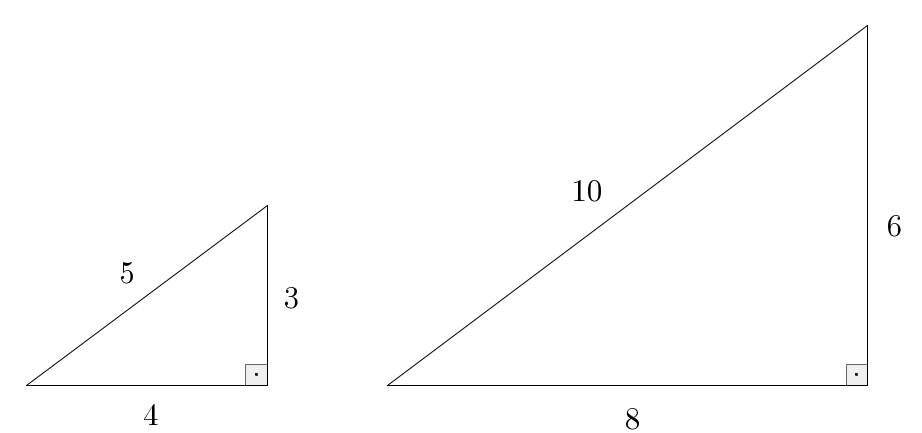
\includegraphics[scale=.3]{/figures/9-1-1-intro.png}
%\end{figure}
%
%The dotted square symbol is a shorthand for ``$90^\circ$ degrees''. Triangles which have a $90^\circ$ angle are called {\bf right triangles}, and will be the main focus of our discussion. What do similar triangles actually have in common? Certainly angles, but not necessarily the lengths of the sides. However, the {\bf ratios} between any two sides of a triangle will remain the same, no matter how the triangle gets rescaled. Such ratios ultimately give us so much information about the given right triangle that they deserve special names: sine, cosine, and tangent.
%
%
%\section{Definitions and examples}
%
%\begin{callout}
%  {\bf Definition (right triangle trig):} Consider the following right triangle, with one angle $\theta$ (this is the lowercase greek letter ``theta'') indicated, and sides labeled $a$, $b$ and $c$.
%
%\begin{center}
%  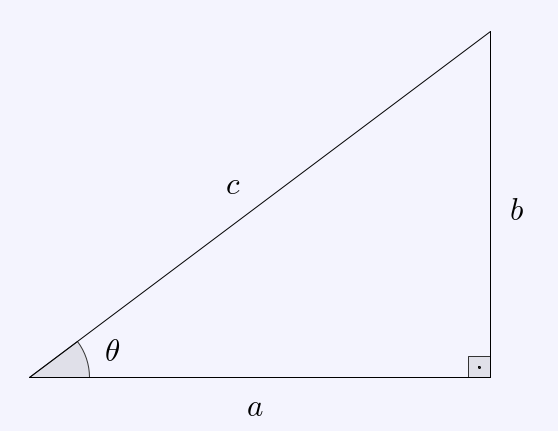
\includegraphics[scale=.3]{/figures/9-1-1-defn.png}
%\end{center}
%  
%  Then:
%  \begin{itemize}
%  \item   The side labeled with $a$ is called the {\bf adjacent} side to $\theta$.
%  \item The side labeled with $b$ is called the {\bf opposite} side to $\theta$.
%  \item   The side labeled with $c$ is called the {\bf hypotenuse} of the triangle.
%  \end{itemize}
%  With this in place, we define the {\bf sine}, {\bf cosine}, and {\bf tangent} of $\theta$, by $$\sin\theta = \frac{b}{c} \left(= \frac{\rm opp.}{\rm hyp.}\right), \quad \cos\theta = \frac{a}{c}\left(=\frac{\rm adj.}{\rm hyp.}\right), ~~\mbox{and}~~ \tan\theta = \frac{b}{a} \left(= \frac{\rm opp.}{\rm adj.}\right).$$
%\end{callout}
%
%\begin{remark}
%  The hypotenuse of a right triangle is always the side opposite to the right angle. Also note that $\tan\theta = \sin\theta/\cos\theta$. You might have seen the mnemonic ``SOH CAH TOA'' before: for example, ``SOH'' means ``sine equals opposite over hypotenuse'', and so on.
%\end{remark}
%
%\begin{example}
%  For each of the following triangles with given angle $\theta$, identify the adjacent (adj.), opposite (opp.) and hypotenuse (hyp.), and compute $\sin\theta$, $\cos\theta$ and $\tan\theta$.
%
%  \begin{enumerate}[label=\alph*.]
%  \item  \begin{figure}[h]
%  \centering
%  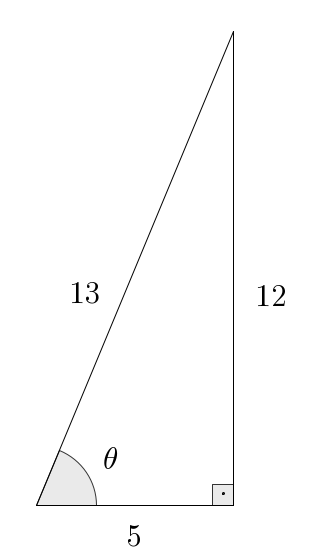
\includegraphics[scale=.3]{/figures/9-1-1-triangle-5-12-13.png}
%\end{figure}
%
%
%    \begin{explanation}
%      We have ${\rm opp.} = 12$, ${\rm adj.} = 5$ and ${\rm hyp.} = 13$. This means that $$\sin\theta = \frac{12}{13}, \quad \cos\theta = \frac{5}{13},\quad \mbox{and}\quad \tan\theta = \frac{12}{5}.$$
%    \end{explanation}
%    
%  \item \begin{figure}[h]
%  \centering
%  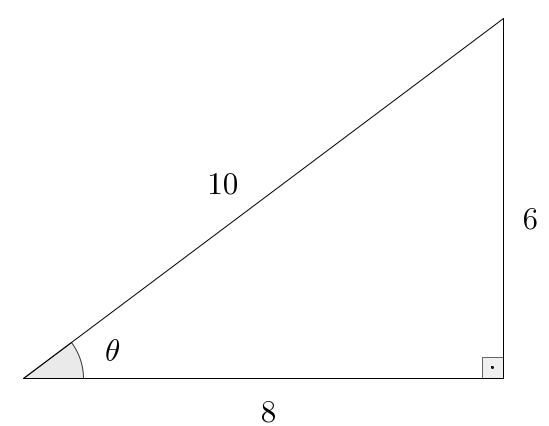
\includegraphics[scale=.3]{/figures/9-1-1-triangle-6-8-10.png}
%\end{figure}
%
%    \begin{explanation}
%      We have ${\rm opp.} = 8$, ${\rm adj.} = 6$ and ${\rm hyp.} = 10$. This means that $$\sin\theta = \frac{8}{10}=\frac{4}{5}, \quad \cos\theta = \frac{6}{10}=\frac{3}{5},\quad \mbox{and}\quad \tan\theta = \frac{8}{10}=\frac{4}{3}.$$
%    \end{explanation}
%    
%  \item \begin{figure}[h]
%  \centering
%  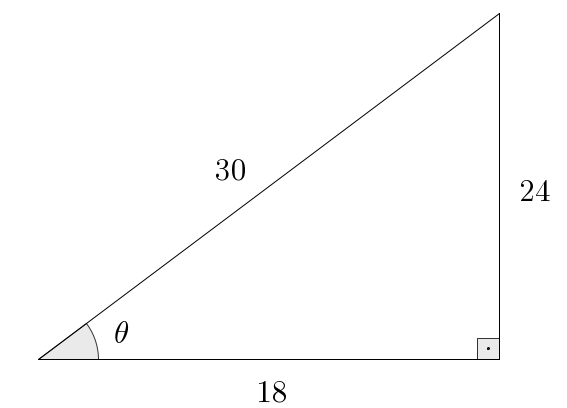
\includegraphics[scale=.3]{/figures/9-1-1-triangle-18-24-30.png}
%\end{figure}
%
%
%        \begin{explanation}
%          We have ${\rm opp.} = 24$, ${\rm adj.} = 18$ and ${\rm hyp.} = 30$. This means that $$\sin\theta = \frac{24}{30}=\frac{4}{5}, \quad \cos\theta = \frac{18}{30}=\frac{3}{5},\quad \mbox{and}\quad \tan\theta = \frac{24}{18}=\frac{4}{3}.$$ Note that the values were the same values as in the previous item. This was expected, as the triangle there is similar to the triangle given here (the scaling factor is $3$).\end{explanation}    
%  \end{enumerate}
%\end{example}
%
%\begin{remark}
%  Note that in all of the above examples, the values of $\sin\theta$ and $\cos\theta$ were always less than $1$. This is always true, and a general consequence of the fact that the hypotenuse is always bigger than either of the other two sides.
%\end{remark}
%
%Often, one has information about the angles, but not about all the sides. Knowing $\sin\theta$, $\cos\theta$ and $\tan\theta$ helps us find out missing sides of a given right triangle. For that, the following fact is extremely important:
%
%\begin{callout}
%  {\bf Theorem (Fundamental Identity):} For any given angle $\theta$, we have that $$\sin^2\theta + \cos^2\theta =1.$$Here, $\sin^2\theta$ means $(\sin\theta)^2$, and similarly for $\cos^2\theta$.
%\end{callout}
%
%Why is this true? Consider again a right triangle like below:
%
%\begin{figure}[h]
%  \centering
%  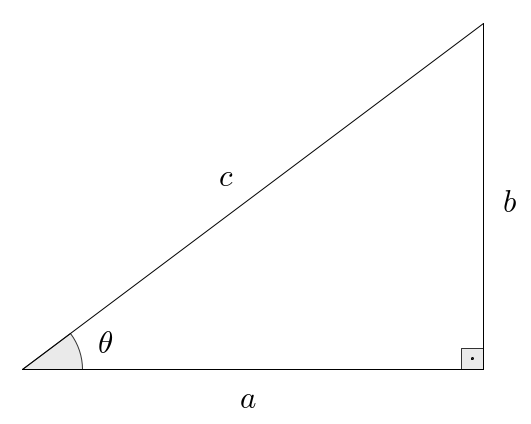
\includegraphics[scale=.3]{/figures/9-1-1-identity.png}
%\end{figure}
%
%
%Then we know that $\sin\theta = b/c$ and $\cos\theta = a/c$. But the Pythagorean theorem also says that $a^2+b^2=c^2$. Putting all of this together, we have that $$\sin^2\theta + \cos^2\theta = \left(\frac{b}{c}\right)^2 + \left(\frac{a}{c}\right)^2 = \frac{b^2}{c^2}+\frac{a^2}{b^2} = \frac{a^2+b^2}{c^2} = \frac{c^2}{c^2} = 1,$$as required.
%
%Let's see how to apply this.
%
%\begin{example}For each of the following triangles, given the value of a trigonometric function at the indicated angle $\theta$, find the lengths of the missing sides.
%  \begin{enumerate}[label=\alph*.]
%  \item Given: $\sin\theta = \sqrt{2}/6$ on
%
%    \begin{figure}[h]
%      \centering
%      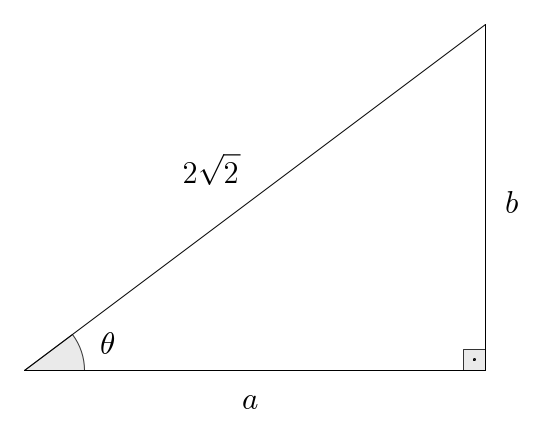
\includegraphics[scale=.3]{/figures/9-1-1-triangle-sin-2sqrt2-6.png}
%    \end{figure}
%
%    \begin{explanation}
% From the given information, we know that $$\frac{\sqrt{2}}{6} = \sin\theta = \frac{b}{2\sqrt{2}} \implies b = \frac{\sqrt{2}\times (2\sqrt{2})}{6} = \frac{2}{3}.$$Now we use the Pythagorean theorem: the relation $a^2 +(2/3)^2=(2\sqrt{2})^2$ gives us that $$a^2+\frac{4}{9} = 8 \implies a^2 = 8-\frac{4}{9} = \frac{68}{9} \implies a = \frac{2\sqrt{17}}{3}.$$Alternatively, to find the value of $a$, we can also use the fundamental identity $\sin^2\theta+\cos^2\theta=1$ to find $\cos\theta$ first --- which then yields $a$. Here's how this goes: $$ \left(\frac{\sqrt{2}}{6}\right)^2+\cos^2\theta=1 \implies \cos^2\theta = 1- \frac{2}{36} \implies \cos^2\theta = \frac{34}{36},$$and so $\cos\theta = \sqrt{34}/6$. Thus $$\frac{\sqrt{34}}{6} = \cos\theta = \frac{a}{2\sqrt{2}} \implies a = \frac{2\sqrt{2} \times \sqrt{34}}{6} = \frac{2\sqrt{17}}{3},$$as it should be. This is not something particular to this example: usually there is more than one strategy to solve this sort of problem. Which one is the best? You'll be the judge.
%    \end{explanation}
%    
%  \item Given: $\cos\theta = \sqrt{3}/7$ on
%
%    \begin{figure}[h]
%      \centering
%      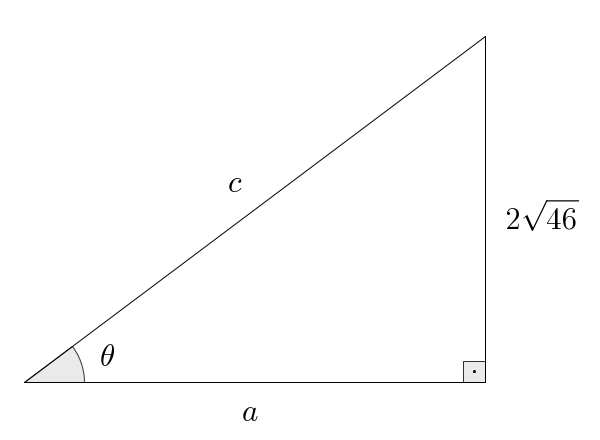
\includegraphics[scale=.3]{/figures/9-1-1-triangle-cos-2sqrt46.png}
%    \end{figure}
%
%    \begin{explanation}
%      Since this time we were given $\cos\theta$, but also the opposite side to $\theta$, which does not appear on the expression for $\cos\theta$, we must rely more on the Pythagorean theorem instead. In any case, we know that $$\frac{\sqrt{3}}{7}= \cos\theta=\frac{a}{c}  \implies c = \frac{7a}{\sqrt{3}}. $$Now, the Pythagorean relation reads $a^2 + (2\sqrt{46})^2 = (7a/\sqrt{3})^2$, and so: $$a^2 + 184 = \frac{49a^2}{3} \implies 184 = \frac{49a^2}{3}-a^2$$Continuing to manipulate this, we see that $$184 = \frac{46a^2}{3} \implies a^2 = \frac{184 \times 3}{46} \implies a^2 = 12 \implies a = 2\sqrt{3}.$$It remains to find the value of $c$. So we go back to the beginning and compute $$c = \frac{7a}{\sqrt{3}}\implies c = \frac{7(2\sqrt{3})}{\sqrt{3}} \implies c=14.$$
%    \end{explanation}
%    
%  \end{enumerate}
%\end{example}
%
%
%\section{Values of trig functions for standard angles}
%
%We know that the sum of the inner angles of a triangle is always $180^\circ$. For right triangles, one of the angles is $90^\circ$, which means that the sum of the remaining two angles must also be $90^\circ$. Frequently we encounter triangles whose angles are $30^\circ$, $60^\circ$ and $90^\circ$, and also triangles whose angles are $45^\circ$, $45^\circ$ and $90^\circ$.
%
%[figure]
%
%These triangles have a special type of symmetry, which we'll exploit to find the values of sine, cosine, and tangent, for $30^\circ$, $45^\circ$ and $60^\circ$. Finding the values of these trig functions for arbitrary angles, by hand, is a very difficult task. We will see later some trigonometric identities that may help us find such values for other angles but, in general, using a calculator (paying close attention to whether it is set to right ``units'') is the way to go.
%
%\subsection{For $30^\circ$ and $60^\circ$}
%
%Consider an equilateral triangle of side length $\ell$. Equilateral means that all the sides have the same length. This implies that all the inner angles must be equal and, since they must add up to $180^\circ$, each of them equals $60^\circ$. But also draw a height $h$:
%
%\begin{figure}[h]
%  \centering
%  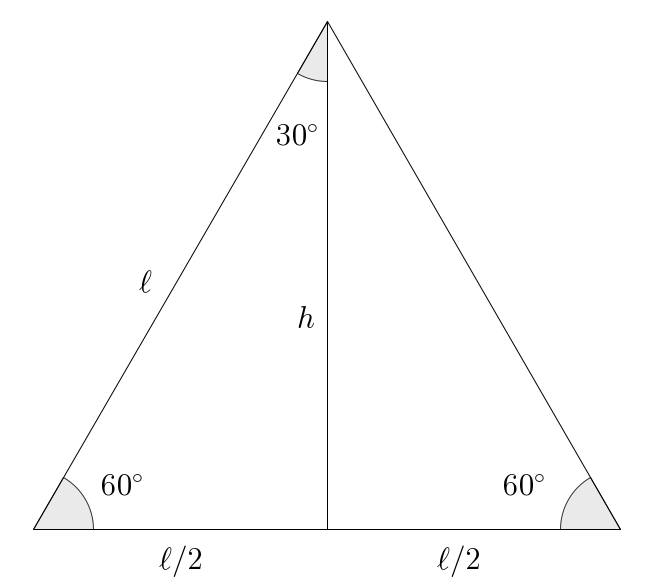
\includegraphics[scale=.3]{/figures/9-1-1-triangle-30.png}
%\end{figure}
%
%By the Pythagorean theorem, we know that $$\ell^2 = \left(\frac{\ell}{2}\right)^2 + h^2,$$and so we may compute: $$\ell^2 = \frac{\ell^2}{4} + h^2 \implies \frac{3\ell^2}{4} = h^2 \implies h = \frac{\ell\sqrt{3}}{2}.$$
%
%Now, relative to the $60^\circ$ angle, we recognize $${\rm opp.} = h = \frac{\ell\sqrt{3}}{2}, \quad {\rm adj.} = \frac{\ell}{2}, \quad\mbox{and}\quad {\rm hyp.} = \ell.$$
%
%This means that $$\sin(60^\circ) = \frac{h}{\ell} = \frac{\left(\frac{\ell\sqrt{3}}{2}\right)}{\ell} = \frac{\sqrt{3}}{2},$$as well as $$\cos(60^\circ) = \frac{\ell/2}{\ell} = \frac{1}{2}\quad\mbox{and}\quad \tan(60^\circ) = \frac{\sin(60^\circ)}{\cos(60^\circ)} = \frac{\sqrt{3}/2}{1/2} = \sqrt{3}.$$
%
%To find the values of $\sin(30^\circ)$, $\cos(30^\circ)$, and $\tan(30^\circ)$, we can use the same triangle, noting that the opposite side to $30^\circ$ is the adjacent side to $60^\circ$, and that the adjacent side to $30^\circ$ is the opposite side to $60^\circ$. Since the hypotenuse is always the side opposite to the right angle, we conclude that $$\sin(30^\circ) = \cos(60^\circ) = \frac{1}{2}, \quad \cos(30^\circ) = \sin(60^\circ) = \frac{\sqrt{3}}{2}$$and, finally, that $$\tan(30^\circ) = \frac{\sin(30^\circ)}{\cos(30^\circ)} = \frac{1/2}{\sqrt{3}/2} = \frac{1}{\sqrt{3}} = \frac{\sqrt{3}}{3}.$$
%
%\begin{remark}
%  This is a general phenomenon: two acute angles are called {\bf complementary} if they add up to $90^\circ$. In other words, the complementary angle to $\theta$ is always $90^\circ - \theta$, and $\sin\theta = \cos(90^\circ - \theta)$, as well as $\cos\theta = \sin(90^\circ - \theta)$. In particular, this justifies the name ``cosine'': it is the sine of the complement. We will discuss ``coterminal angles'' and ``cofunctions'' in more generality later.
%\end{remark}
%
%\subsection{For $45^\circ$}
%
%Consider a square of side length $\ell$, and draw a diagonal $d$.
%
%\begin{figure}[h]
%  \centering
%  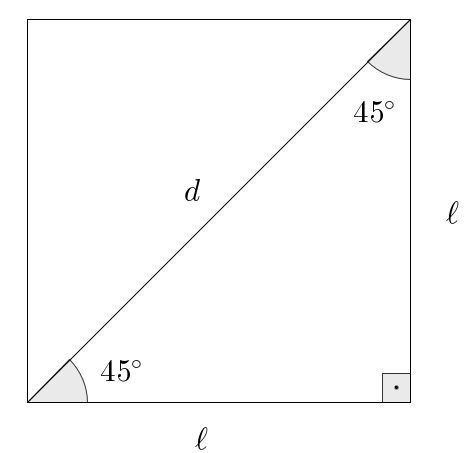
\includegraphics[scale=.3]{/figures/9-1-1-triangle-45.png}
%\end{figure}
%
%By the Pythagorean theorem, $d^2 = \ell^2+\ell^2 = 2\ell^2$ implies that $d=\ell\sqrt{2}$. Relative to either of the $45^\circ$ angles, we have $${\rm opp.} = \ell, \quad {\rm adj.} =\ell, \quad\mbox{and}\quad {\rm hyp.}=d=\ell\sqrt{2}.$$
%Hence $$\sin(45^\circ) =\cos(45^\circ) =  \frac{\ell}{\ell\sqrt{2}} = \frac{1}{\sqrt{2}} = \frac{\sqrt{2}}{2} \quad\mbox{and}\quad \tan(45^\circ) = \frac{\sin(45^\circ)}{\cos(45^\circ)} = 1.$$
%
%\begin{remark}
%  It is convenient to write $\sqrt{2}/2$ instead of $1/\sqrt{2}$ (similarly for $\sqrt{3}/3$ versus $1/\sqrt{3}$), even though the latter is mathematically acceptable, because it makes it easier to estimate. Namely, knowing that $\sqrt{2} \approx 1.414$, we know that $\sqrt{2}/2 \approx 0.707$, but when looking at $1/\sqrt{2}$, what does it mean to divide $1$ by $1.414$? This is the general reason why rationalizing fractions is useful.
%\end{remark}
%
%%\typeout{************************************************}
%%\typeout{Summary}
%%\typeout{************************************************}
%
%\section{Standard values}
%
%We can summarize what we have discovered here in a table. Besides our standard angles of $30^\circ$, $45^\circ$, and $60^\circ$, we can also consider $0^\circ$ and $90^\circ$ as extreme cases. Let's do a quick thought experiment to understand this: if a right triangle had an angle of $0^\circ$, this triangle would in fact collapse to a line segment, and we would have ${\rm opp.} = 0$, while ${\rm hyp}. = {\rm adj}.$, suggesting we set $\sin(0^\circ) = 0$ and $\cos(0^\circ) = 1$. Since $0^\circ$ and $90^\circ$ are complementary, we're forced to set $\sin(90^\circ) = 1$ and $\cos(90^\circ) = 0$. But while $$\tan(0^\circ) = \frac{\sin(0^\circ)}{\cos(0^\circ)} = \frac{0}{1} = 0,$$computing $\tan(90^\circ)$ does not make sense, as we would have a division by $\cos(90^\circ) = 0$. We say that $\tan(90^ \circ)$ is {\bf undefined}, or that it {\bf does not exist} (``DNE'' for short, as usual). So, we have:
%
%$$
%\begin{array}{c||ccccc}
% & 0^\circ & 30^\circ & 45^\circ & 60^\circ & 90^\circ \\
%\hline\hline \\[-1em]  
%\sin \theta & 0 & \frac{1}{2} & \frac{\sqrt{2}}{2} & \frac{\sqrt{3}}{2} & 1 \\[1em]
% \cos \theta & 1 & \frac{\sqrt{3}}{2} & \frac{\sqrt{2}}{2} & \frac{1}{2} & 0 \\[1em]
%\tan\theta& 0 & \frac{\sqrt{3}}{3} & 1 & \sqrt{3} & {\rm DNE}
%\end{array}
%$$
%
%Those values should be committed to heart, but it's easier than what it seems. Here's how you can think about it:
%
%\begin{itemize}
%\item No need to memorize values for tangent: if you know $\sin \theta$ and $\cos \theta$, you can just compute $\tan\theta = \sin \theta/\cos\theta$.
%\item No need to memorize the values for cosine: recall that the cosine of an angle is the sine of the complement. So if you know values for sine, you're in business.
%\item How to memorize values for sine? The one thing you should remember here is that the values $0$, $1/2$, $\sqrt{2}/2$, $\sqrt{3}/2$ and $1$ will appear. What is their order? Simple: write them in increasing order, just like the angles from $0^\circ$ to $90^\circ$. So $$\sin(0^\circ) = 0, ~ \sin(30^\circ) = \frac{1}{2}, ~ \sin(45^\circ) = \frac{\sqrt{2}}{2}, ~ \sin(60^\circ) = \frac{\sqrt{3}}{2}, ~ \sin(90^\circ)=1.$$
%\end{itemize}
%
%\begin{summary}\begin{itemize}
%\item We have defined sine, cosine, and tangent, as ratios between sides of a right triangle. For each angle $\theta$, the fundamental identity $\sin^2\theta+\cos^2\theta=1$ holds. It can be used together with the Pythagorean Theorem to get information about all sides of a given triangle, when some of them might be missing, provided you have some information about the angles.
%\item We have established the standard values of sine, cosine, and tangent, for the most frequent angles of $30^\circ$, $45^\circ$, and $60^\circ$. Those values have been organized in a table. They are so frequent that knowing the values there by heart is useful, but exaggerated efforts into memorizing the table should not be wasted --- understanding how the values are deduced pays off more in the long run.
%\end{itemize}\end{summary}
%



\end{document}
